\chapter{Analisi delle performance delle implementazioni realizate}
\label{ChPerf}

Ho effettuato un analisi delle performance ottenute nelle varie implementazioni 
realizzate per Sp3MM con un insieme eterogeno di matrici di input.\\
Le perstazioni confrontate sono ottenute da valori mediati su 40 ripetizioni
dalle varie implementazioni e configurazioni realizzate per Sp3MM descritte precedentemente.\\
I dati sono stati raccolti mediante un programma di test ( \verb|Sp3MM_test.c| ) automatizzando
l'esecuzione di tutte le implementazioni realizzate dato un set di matrici di input.
I log del programma di test sono stati parsati ed analizzati mediante la libreria di analisi Pandas \cite{pandasMan}.\\
Tutti i test sono stati effettuati sul server dell'Ateneo, caratterizato dai seguenti parametri:
\begin{itemize}
	\item	 OS:	CentOS Stream 8
	\item	CPU:	Intel Xeon Silver 4210 2.20 GHz 40 core
	\item	RAM:	64GB
\end{itemize}

\section{Matrici di input utilizzate}
Il problema originario risolto è un sistema lineare ottenuto da 
una discretizzazione alle differenze finite 
di una PDE di secondo ordine,
utilizzando una griglia regolare e le condizioni al contorno di Dirichlet.\\ %(corrispondente al programma di test di PSBLAS).
Le matrici sparse utilizzate nei test
sono relative ai tripli prodotti di Galerkin in due configurazioni
di generazione degli aggregati in AMG4PSBLAS:
\emph{VanekBrezina} e \emph{Matching}, entrambe con e senza un operazione di smoothing associata.\\
Le caratteristiche del problema di partenza da cui sono derivate i gruppi di matrici,
comportano un pattern di sparsità degli elementi non zero di tipo diagonale 
come è possibile nelle figure seguenti.\\
%matchingMediumSmoothed_UnSmoothed.png  matchingMediumSmoothed_UnSmoothed.ppm.png  varnekBenzina_MediumSmoothed_UnSmoothed.png  varnekBenzina_MediumSmoothed_UnSmoothed.ppm.png

\begin{figure}[H]
  \centering \includegraphics[width=\linewidth,keepaspectratio]{sparseMatrices/matchingMediumSmoothed_UnSmoothed.png}
  \caption{rappresentazione degli elementi \nnz di matrici ottenute con il metodo Matching, con opzione smoothed a sinistra, unsmoothed a destra}
  \decoRule \label{fig:sparseMatrix}
\end{figure}
\begin{figure}[H]
  \centering \includegraphics[width=\linewidth,keepaspectratio]{sparseMatrices/varnekBenzina_MediumSmoothed_UnSmoothed.png}
  \caption{rappresentazione degli elementi \nnz di matrici ottenute con il metodo VanekBrezina, con opzione smoothed a sinistra, unsmoothed a destra}
  \decoRule \label{fig:sparseMatrix1}
\end{figure}
\label{inputClasses}
Data l'eterogeneità degl'input utilizzati, 
ho raggruppato le matrici di test in quattro gruppi in base alla tecnica di generazione degli aggregati %(ovvero le matrici R e P nel prodotto di Galerkin)
e l'uso dello dello smoothing.\\
I gruppi di input utilizzati sono quindi: 
\begin{enumerate}
	\item VarnekBenzina,Smoothed
	\item VarnekBenzina,Unsmoothed
	\item Matching,Smoothed
	\item Matching,Unsmoothed
\end{enumerate}

\section{Configurazioni considerate}
Tra i svariati parametri configurabili a compile-time o a run-time, è stata effettuata 
un analisi di tutte le implementazioni realizzate variando:
\newcounter{queriesCounter}
\begin{enumerate}
	\item	il tipo assegnamento ai thread dello spazio intermedio in implementazioni basate su UpperBound 
	\item	la dimensione delle bitmap utilizzate in alcune implementazioni del prodotto simbolico %(descritte in \ref{chSpMMSymb:structFlagSet})
	\item	il numero di thread da utilizzare 
	\item	il tipo di scheduling openMP, static o dynamic adattato (descritto in \ref{chSpMMAux:dynChunkFairAdapting})
	\setcounter{queriesCounter}{\value{enumi}}
\end{enumerate}
Inoltre, sono state determinate le performance:
\begin{enumerate}
	\setcounter{queriesCounter}{\value{enumi}}
	\item	di ogni implementazione, con configurazione ottimale, per ogni categoria di input (descritte in \ref{inputClasses})
	\item	della migliore implementazione per ogni input, confrontadole con le performance ottenute con un implementazione seriale di riferimento
\end{enumerate}
Altri parametri, come la griglia di partizionamento utilizzata, sono determinate automaticamente in base al numero di thread configurato,
come descritto in \ref{chSpMMAux:ompGrid}.
In particolare per implementazioni bidimensionali, la griglia di partizionamento impiegata è stata determinata con l'approccio
basato sulla funzione \verb|MPI_Dims_create|, descritto in \ref{ompiDimsCreate}.\\
\begin{figure}[H]
  \centering 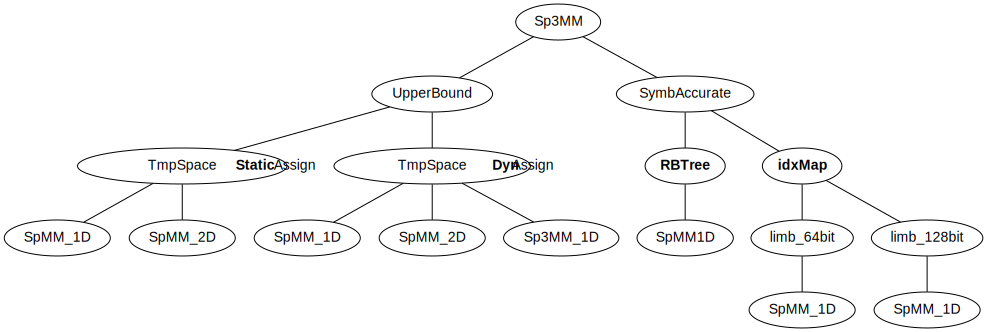
\includegraphics[width=\linewidth,keepaspectratio]{Sp3MM_treeMinimal.dot.txt.png}
  \caption{Diagramma riassuntivo delle varie configurazioni delle implementazione realizzate considerate nei test}
  \decoRule \label{fig:q1}
\end{figure}
\voidLine
Tutti i test nel seguito ad eccezione di quelli menzionati nella sezione \ref{chPerf:multiThread}, sono stati effettuati 
con il numero massimo di thread possibili, ovvero 40 sull'ambiente di esecuzione utilizzato.\\


\section{Determinazione della migliore configurazione}	\label{bestConf}
Nel seguito viene determinata la migliore configurazione, mediando le performance misurate dalle implementazioni relative alle configurazioni considerate,
su tutti gli input disponibili e tutti i tipi di scheduling openMP

\subsection{Migliore assegnamento di spazio intermedio per implementazioni UpperBound}
Come analizzato in \ref{chSpMMSymb:UB_VS_SYMBACC}, implementazioni parallele di SpMM basate su una fase simbolica di tipo UpperBound,
necessitano inevitabilmente di uno spazio temporaneo per i risultati intermedi, 
che ho pre-allocato al blocco di esecuzione parallelo 
ed assegnato ai thread in modo statico o dinamico, 
come descritto in \ref{chSpMMNum:preSplitAS_JA_tmp} ed approfondito in \ref{chSpMMAux:atomicSegAssign}.\\

\begin{figure}[H]
  \centering 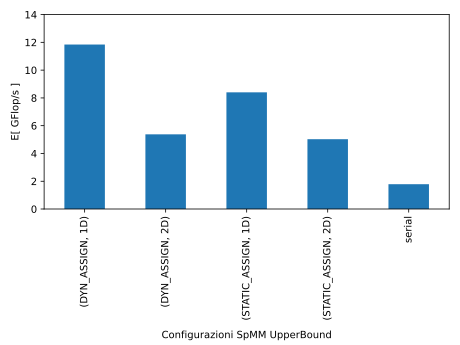
\includegraphics[width=\linewidth,keepaspectratio]{graphs/q1.svg.png}
  \caption{Confronto tra le perfomance medie delle implementazioni UpperBound di SpMM, su tutti gli input considerati, in base a
		tipo di assegnamento dello spazio intermedio ai thread (statico o dinamico) e al tipo di implementazione usata 
		( con partizionamento del lavoro 1D o 2D ) }
  \decoRule \label{fig:q1}
\end{figure}

Come è possibile vedere nella figura \ref{fig:q1}, un assegnamento dinamico dello spazio intermedio ai thread da dei vantaggi
per implementazioni monodimensionali, mentre ha performance pressochè simili nel caso di implementazioni bidimensionali.\\

\subsection{Migliore dimensione delle bitmap per implementazioni con prodotto simbolico accurato}
La versione del prodotto simbolico accurato basata su bitmap di indici, descritta in \ref{chSpMMSymb:structFlagSet} 
ed approfondita in \ref{chSpMMAux:bitmapInsert}, prevede l'uso di un vettore di variabili di tipo \verb|limb_t|
di dimensione configurabile a tempo di compilazione con la macro \verb|LIMB_T|.\\

\begin{figure}[H]
  \centering 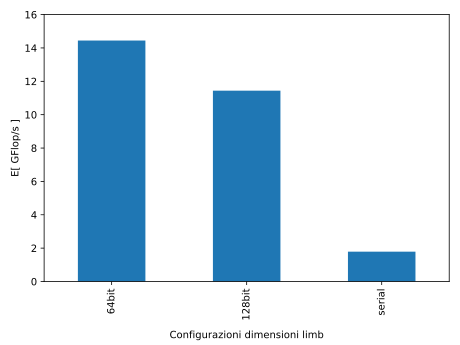
\includegraphics[width=\linewidth,keepaspectratio]{graphs/q2.svg.png}
  \caption{Confronto tra le perfomance medie di Sp3MM con fase simbolica accurata mediante bitmaps di indici,
		   su tutti gli input considerati, variando la dimensione delle singole bitmap tra 64 e 128 bit}
  \decoRule \label{fig:q2}
\end{figure}
Dalla figura \ref{fig:q2} è possibile notare come usare bitmap di 64 bit può può fornire un vantaggio prestazionale
rispetto all'uso di bitmap a 128 bit.

\section{Migliore implementazione per classe di input} \label{chPerf:q3}
Considerando la miglior configurazione determinata in \ref{bestConf}, ho effettuato un confronto delle prestazioni medie
delle varie implementazioni di Sp3MM per ogni classe di input disponibile ( descritte precedentemnte in \ref{inputClasses} )
%\centering \includegraphics[width=\linewidth,keepaspectratio][[width=\linewidth,keepaspectratio]{q3.svg.png}
\begin{figure}[H]	
  \centering 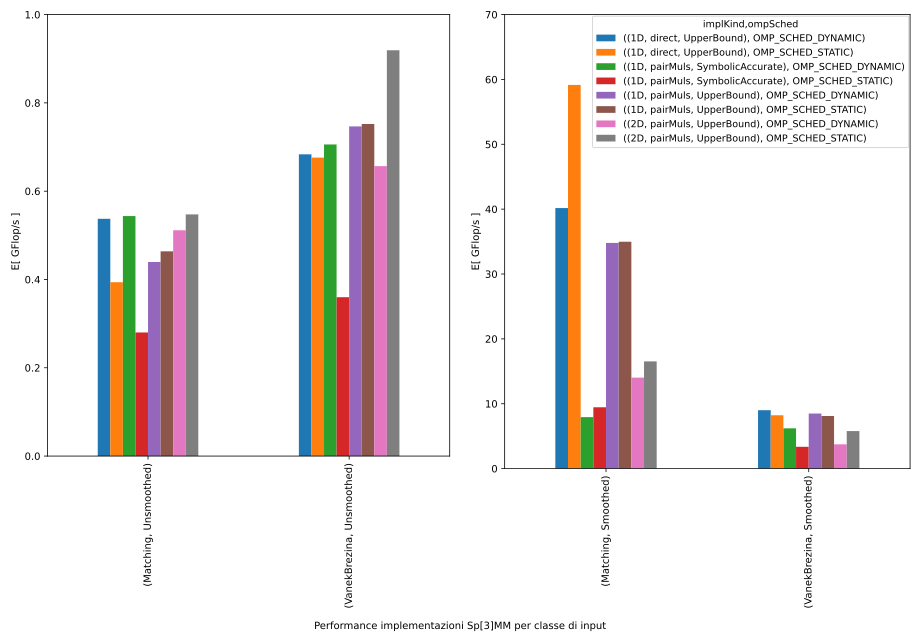
\includegraphics[width=\linewidth,keepaspectratio]{graphs/q3.svg.png}
  \caption{Confronto tra le perfomance medie della miglior configurazione per le implementazioni di Sp3MM per ogni classe di input}
  \label{fig:q3}
\end{figure}
Come è possibile notare dalla figura \ref{fig:q3}, si hanno performance molto diverse in base alla classe di input considerata.
In particolare, le implementazioni su matrici di tipo \emph{Unsmoothed} soffrono di prestazione nettamente inferiori di quelle 
su matrici \emph{Smoothed}.\\
Le implemenetazioni con performance migliori variano tra le classi di input considerate, tuttavia è possibile osservare che:
\begin{itemize}
	\item il triplo prodotto diretto dia prestazioni migliori degli altri in tutte le classi salvo \emph{VarnekBenzina,Unsmoothed}.
	\item la configurazione di scheduling openMP static sembra dare prestazioni migliori per le implementazioni bidimensionali,
		  viceversa la controparte dynamic con adattato dei chunk da risultati migliori per implementazioni monodimensionali e per il triplo prodotto diretto.
	\item le implementazioni monodimensionali UpperBound performano meglio di quelle bidimensionali nelle classi di input \emph{Smoothed},
		  viceversa per le classi \emph{Unsmoothed}
\end{itemize}

\section{Guadagno di performance rispetto ad una implementazione seriale} \label{chPerf:allMatrixs}
Come precedentemente analizzato le prestazioni di Sp3MM sono molto variabili in base al tipo di input, 
l'implementazione utilizzata e la configurazione applicata.\\
Per questo motivo ho deciso di misurare il vantaggio prestazionale ottenuto dalla migliore implementazione parallela 
rispetto ad una implementazione seriale di riferimento ( descritta in \ref{implSerialeRiferimento} ).\\
\begin{figure}[H]
  \centering 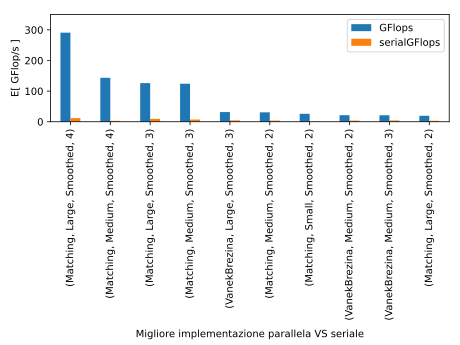
\includegraphics[width=\linewidth,keepaspectratio]{graphs/q4-b.svg.png}
  \decoRule \label{fig:q4big}
\end{figure}
\begin{figure}[H]
  \centering 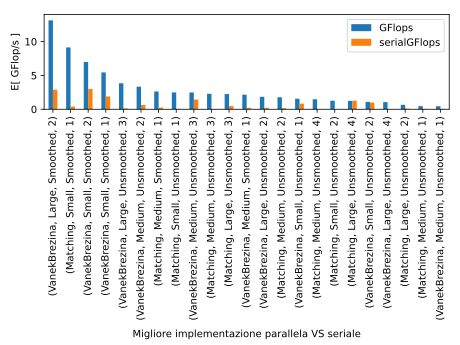
\includegraphics[width=\linewidth,keepaspectratio]{graphs/q4-s.svg.png}
  \decoRule \label{fig:q4small}
\end{figure}
Come è possibile notare dai grafici \ref{fig:q4big}, \ref{fig:q4small}, le implementazioni 
parallele di Sp3MM performano meglio dell'implementazione seriale per la stragrande maggioranza dei casi,
in misura variabile in base all'input considerato.\\

\section{Performance variando il numero di thread}	\label{chPerf:multiThread}
La dimensione delle matrici di input e il loro pattern di sparsità,
potrebbe comportare che le performance migliori per Sp3MM sono ottenute con un numero di thread diverso da quello massimo possibile.\\
Per questo motivo ho effettuato un analisi delle prestazioni misurate per alcune esecuzioni di Sp3MM
al variare del numero di thread.\\
\begin{figure}[H]
  \centering 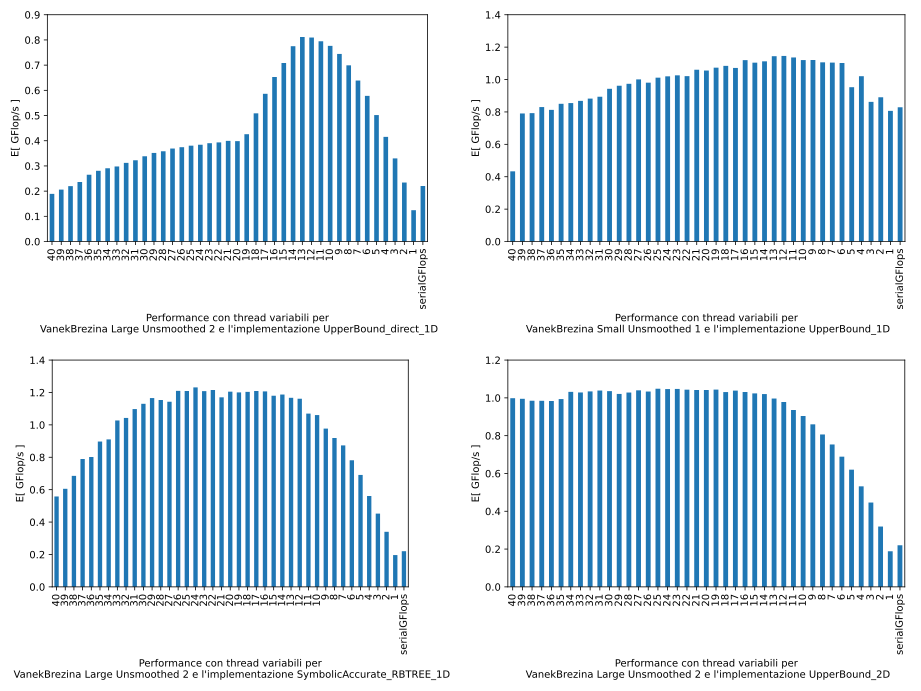
\includegraphics[width=\linewidth,keepaspectratio]{graphs/q5.svg.png}
  \caption{performance misurate su alcune esecuzioni di Sp3MM, variando il numero di thread impiegati}
  \decoRule \label{fig:q5}
\end{figure}
Come è possibile notare dai grafici \ref{fig:q5}, è possibile avere un guadagno di performance 
abbassando il grado di parallelismo, in misura differente in base all'implementazione e alla matrice considerata.\\

\section{Conclusioni}
Di seguito alcune considerazioni che è possibile trarre dalle analisi delle performance effettuate.\\
%TODO gestione registri a 128 bit VS 64 ??
In generale, il pattern di sparsità dei valori \nnz delle matrici di input può causare uno sbilanciamento
nelle porzioni di lavoro assegnate ai thread in misura differente in base:
\begin{itemize}
	\item	all'approccio di divisione del lavoro usato,
	\item	alla tipologia di implementazione usata (triplo prodotto diretto o uso di una fase simolica accurata)
	\item	al tipo di scheduling openMP usato così come altre configurazioni
\end{itemize}
Uno sbilanciamento del carico di lavoro comporta un cattivo uso delle risorse computazionali, causando un peggioramento delle performance 
come come è possibile notare nell'analisi effettuate in \ref{chPerf:q3}.\\
\voidLine
Il livello di parallelismo usato può influire molto sulle performance, come visibile nell'analisi effettuata in \ref{chPerf:multiThread},
sia per le ragioni appena citate che per motivi legati all'overhead di schedulare un alto numero di thread
per input piccoli.
\voidLine
L'overhead complessivamente introdotto da openMP può in generale comportare un costo superiore al beneficio
ottenuto dall'esecuzione parallela per alcuni input, come visibile in pochi casi in \ref{fig:q4small}.
Inoltre, in \ref{fig:q5} è possibile notare uno svantaggio prestazionale in alcune esecuzioni parallele con un solo thread
rispetto all'esecuzione dell'implementazione seriale di riferimento, 
probabilmente dovuto all'overhead di inizializzazione e scheduling di openMP.\\

